\documentclass[letterpaper, 10 pt, conference]{ieeeconf}

\IEEEoverridecommandlockouts                              % This command is only needed if 
                                                          % you want to use the \thanks command

\overrideIEEEmargins                                      % Needed to meet printer requirements.

\pdfobjcompresslevel=0
%\pdfminorversion=4

% See the \addtolength command later in the file to balance the column lengths
% on the last page of the document
\usepackage{graphicx}
\usepackage{xcolor}
\usepackage{epstopdf}
%
\let\proof\relax
\let\endproof\relax            % hacks needed to prevent redefining of \proof \endproof elsewhere
% math packages
\usepackage{amsthm}
\usepackage{amsmath}
\usepackage{amssymb}
\usepackage{algorithm, algpseudocode}  %algorithmic
%
\usepackage{tikz}
\usepackage{siunitx}
\usepackage{booktabs}
\usepackage{multirow}
\usepackage{subfig}
\usepackage{pdfpages}
\usepackage{cite}
%\usepackage[showframe]{geometry} %Full width figures
\setlength\arraycolsep{1.5pt}
% ------- theorem/definition/lemma/prop definitions ----- %
\newtheorem{theorem}{Theorem}
\newtheorem{corollary}{Corollary}[theorem]
\newtheorem{lemma}[theorem]{Lemma}
\newtheorem{prop}[theorem]{Proposition}

\theoremstyle{definition}
\newtheorem{definition}[theorem]{Definition}

%% ----- Macro to leave a boxed "note" in the text ------ %%
\newcommand{\note}[2][NOTE]{\vspace{3 mm}\par \noindent \framebox{\color{red} \begin{minipage}[c]{1.0 \hsize} {\bf #1:} #2 \end{minipage}}\vspace{3 mm}\par}
%\newcommand{\note}[1]{}
\newcommand{\etal}{\textit{et al}.}
\newcommand{\ie}{\textit{i}.\textit{e}. }
\newcommand{\eg}{\textit{e}.\textit{g}. }
%
\newcommand{\Cs}{\mathcal{C}}
\newcommand{\Ns}{\mathcal{N}}
\newcommand{\Os}{\mathcal{O}}
\newcommand{\Ps}{\mathcal{P}}
\newcommand{\Rs}{\mathcal{R}}
\newcommand{\Ss}{\mathcal{S}}
\newcommand{\Ws}{\mathcal{W}}

% declare argmax, argmin
\DeclareMathOperator*{\argmax}{arg\,max}
\DeclareMathOperator*{\argmin}{arg\,min}

\graphicspath{ {./Figures/} }

\setlength{\voffset}{0.055in}

%%% ------------------------------------------------------------------------- %%
\newcommand{\cell}{\mathcal{C}}
%%% ------------------------------------------------------------------------- %%
\title{\LARGE \bf From Multi-Target Sensory Coverage to Complete Sensory Coverage: An Optimization-Based Robotic Sensory Coverage Approach}

\author{Joel W. Burdick, Amanda Bouman, Elon Rimon \thanks{Engineering and Applied Sciences, California Institute of Technology, Pasadena, CA 91125, \texttt{\{abouman,jburdick\}@caltech.edu}}}

\begin{document}
\maketitle
\thispagestyle{empty}
\pagestyle{empty}

%%% ------------------------------------------------------------------------------------------ %%
\begin{abstract}

This paper considers progressively more demanding off-line robotic sensory coverage problems in an optimization framework.  In the first problem, a robot finds the shortest path to cover a set of target nodes with its sensors. We formulate this problem as a mixed integer nonlinear optimization problem. Because this problem is NP-hard, we develop a polynomial-time approximation algorithm with a bounded approximation ratio.
The next problem concerns sensory coverage
%Next we develop a novel version of the problem 
that takes advantage of the possibility to view multiple targets from a single location. 
%While approximation is an inappropriate notion for this %problem, 
Extension of our coverage  
approach 
%provides a novel polynomial-time approximation algorithm
provides a polynomial-time approximation algorithm that simplifies the coverage path geometry.  Finally, we show how the complete sensory coverage problem can be formulated as an optimization problem over a decomposition of a given region into convex polygons.  Extension of the previously introduced heuristics provides a polynomial time solution with bounded approximation.  Examples illustrate the methods.
\end{abstract}


%%% ------------------------------------------------------------------------------------------ %%
\section{Introduction} \label{sec:intro}

\noindent This paper considers a family of off-line robotic sensory coverage problems that derive from the {\em covering path problem} (CPP)
\cite{current_covering_1989,current_efficient_1994,arkin_approximation_1994}, which has been little considered in the robotics community.  In the basic problem setting, a mobile robot must select the {\em shortest} path, $\mathcal{P}^{*}$, which allows its sensors to cover $n$ {\em target nodes} from views along $\mathcal{P}^*$.  Unlike the classical {\em watchman problem} \cite{urrutia_art_2000,danner_randomized_2000}, the robot's sensing range is a convex region, $R$, and  the robot's motion cost is considered.  Other advantages are described below.

There are several CPP variations.  In the {\em covering tour} version, the robot starts at a {\em depot} location, finds the shortest closed path that covers each target, and returns to the depot.  In the {\em s-t-CPP} problem
\cite{hoogeveen_analysis_1991}, the robot starts at node $N_1$, and must find the shortest path to cover nodes $N_2,\ldots,N_{n-1}$, while ending within the sensor range of $N_n$. In the {\em s-CPP} version, the robot starts at $N_1$, and finds a shortest covering path that ends within the sensing region associated to any node (except $N_1$).  This paper focuses on the {\em s-t-CPP}, but the methods can be readily adapted to the other variants.

This work is motivated by our participation \cite{AutoSpot} in the DARPA Subterranean challenge (www.subtchallenge.com): a  competition where robot teams rapidly navigate and map a priori unknown underground environments with the goal of locating objects of interest. The competition environments (e.g. tunnels and caves) are characterized by complex topologies with uneven and obstacle-laden terrain. Many coverage planning algorithms are ill-suited to these environments, as they assume rectilinear workspace boundaries or decomposition of space into uniform cells \cite{joon_seop_oh_complete_2004,gonzalez_bsa:_2005}. 

%%% ------------------------------------------------------------------------------------------ %%

{\bf Relation to Previous Work.}  Coverage planning is an established sub-discipline of robotic motion planning. Detailed surveys by Bormann~\cite{bormann_indoor_2018}, Choset ~\cite{choset_coverage_2001} and Galceran~\cite{galceran_survey} categorize various coverage problems and review coverage planning methods.  Coverage planning has been deployed for many worthwhile applications \cite{?,?}. 

While the ultimate goal of this research program is on-line sensory coverage \cite{zelinsky_planning_1993,?,?}, the present paper focuses on off-line planning of sensor coverage paths.  This problem is also known as the inspection problem \cite{?,?z}.  Many off-line coverage planning and inspection algorithms have been introduced \cite{?,?,?}.  While this paper introduces novel algorithms, its primary contributions focus on exposing the fundamental optimization underpinnings of shortest path sensory coverage, and establishing competitive approximation bounds for this class of problems.  While the CPP formulation (Section \ref{sec:covering_path}) as a mixed integer nonlinear program  (MINLP) is not new \cite{current_covering_1989,current_efficient_1994,golden_generalized_2012}, we introduce this useful problem to the robotics literature. Because it is NP-hard, Section \ref{sec:polynomial} develops a new polynomial time algorithm, and a novel bound on the algorithm's approximation ratios that is  better than prior results from the computational geometry literature.  The entirely novel MINLP formulation (Section \ref{sec:fewer}) sheds light on the algorithmic problem of viewing multiple targets from a single view, in order to improve coverage efficiency. Our formulation of the complete sensory coverage task as a MINLP (Section \ref{sec:complete_coverage}) and its polynomial time approximation are also completely new.

In the most related work, Englot and Plover \cite{englot_three-dimensional_2013,christensen_planning_2017} used sample-based methods and Christofides' Traveling Salesman Problem Heurstic (from which the Hoogeveen heuristic in Section \ref{sec:Hoogeveen} is derived) to plan impressive 3-dimensional (3D) inspection tours of surfaces.  They also present a polynomial time algorithm to prune unnecessary sensing actions (like our Section \ref{sec:overlap_heuristic}). Similarly, Bircher et. al \cite{bircher_3D} use the Held Karp TSP heuristic and viewpoint optimization to plan equally impressive aerial inspections of surfaces in 3D. While our work at present only applies to 2D surfaces, these prior efforts did not expose the formal optimization framework of our Problems $\# 1$, $\#2$, and $\# 3$.  Nor do they offer any performance characterizations of their algorithms, like our Propositions \ref{prop:bound1}, \ref{prop:bound_overlap}, and \ref{prop:final}.  

An optimization approach to coverage has practical advantages.  For complete sensory coverage, our formulation allows for irregular convex
decomposition of the space to be covered, providing a flexible problem solving framework. The connection to NP-hard optimization problems motivates the adoption of concepts from the approximation algorithm literature \cite{arkin_approximation_1994}.  The formulation of the fundamental optimization geometry of coverage planning will allow future integration of effects, such as robot dynamics and sensor uncertainty, into the coverage planning process, as these concerns can be formulated as optimization costs or constraints.
% Alternative Phrasing: Formulating the coverage planning problem as a fundamental geometric optimization also allows for higher fidelity consideration of the world and robot state, such as robot dynamics and sensor uncertainty, through integration of optimization costs and constraints.


%%% ------------------------------------------------------------------------------------------ %%
\section{The Multi-Target Sensory Coverage Problem }\label{sec:covering_path}

\noindent Consider a planar mobile robot.  Let $\mathcal{F}_W$ denote a reference frame fixed in the plane. Reference frame $\mathcal{F}_B$ fixed to the robot defines its coordinates, $q=(x,y,\theta)$, relative to $\mathcal{F}_W$.  The robot sensors can cover a {\em sensing region}, $R$.  This region is assumed to be a circle, a convex polygon, or %a convex 
a~union of such shapes (see Fig. \ref{fig:sensing_region}, and Eqs (\ref{eq:quadratic})-(\ref{eq:polytope})).  We let $R(q)$ denote the region of the plane that can be sensed when the robot lies at $q$.  We mainly focus on circular covering sensors, which render the robot's orientation irrelevant.  For polygonal sensing regions, the problem depends upon the robot's orientation, $\theta$. But if $r_{max}$ defines the maximum sensor range, the sensing constraint can be similarly defined by a circle with radius $r_{max}$, since some robot orientation will allow the target to be sensed at range $r_{max}$.
%
%% ------------------------------ %%
\begin{figure}
  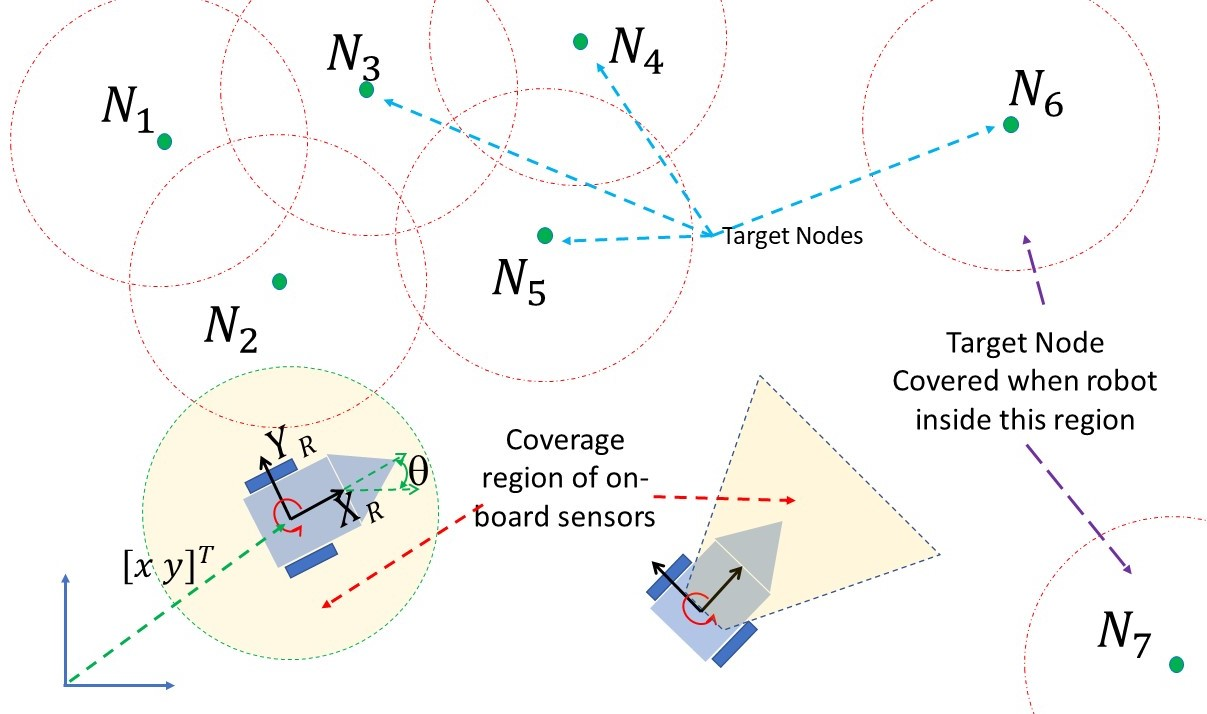
\includegraphics[height=1.8 true in]{ProblemGeometry.jpg}
  \vskip -0.05 true in
  \caption{Diagram of the problem geometry and demonstration of circular and convex polygonal
    robot sensing regions, $R$}
  \label{fig:sensing_region}
    \vskip -0.25 true in
\end{figure}
%% ------------------------------ %%

{\bf Multi-target coverage:} The goal is to find $(m-1)$ {\em sensing configurations} $\mathcal{S} =\{S_2,\ldots,S_m\}$, and a path $\Ps$ starting at $N_1$ that passes through each member of $\Ss$ such that all $(n-1)$ targets are covered by the robot sensors. The sensing locations and their traversal order specify the covering path.

The optimal covering path is the solution to a constrained optimization problem. Moreover, we assume that $m=n$: there are as many sensing nodes as targets. The general case is developed in Section \ref{sec:fewer}.  The covering path minimizes:
  \begin{equation}\label{eq:min_cost}
     Cost =  \ \sum_{i=1}^n \sum_{j=1,j\ne i}^n \xi_{ij}\ d(S_i,S_j)
  \end{equation}
where the {\em incidence variables}, $\vec{\xi}$ for $i,j\in 1,\ldots,m$, are
  \[ \xi_{ij} = \begin{cases} 1 & {\rm when\ target\ } N_j\
                  {\rm is\ covered\ after}\ N_i\ {\rm is\ covered} \\
                              0 & {\rm otherwise} \end{cases} \]
and distance function $d(S_i,S_j)\ge 0$ satisfies the triangle inequality.  This distance can be the Euclidean distance, or the cost of the robot's travel between nodes.  Cost function (\ref{eq:min_cost}) allows for asymmetric costs: i.e., $d(S_i,S_j)\ne d(S_j,S_i)$.  Hereafter we assume symmetric costs: $d(S_i,S_j)=d(S_j,S_i)$ $\forall i,j$.  But our analysis extends to the asymmetric case.

{\bf Obstacles} can be incorporated in two ways. In the first approach a local planner finds an obstacle-free path between $S_i$ and $S_j$, if one exists, and estimates the traversal cost. If no path is feasible, then $\xi_{ij}$ is set to zero. In the second approach, obstacles are modeled  by convex approximations to their boundaries, and included as additional constraints in the following optimization problems.  

For the covering path to be well defined, the minimization of cost (\ref{eq:min_cost}) must be subject to a number of constraints:
%
\begin{enumerate}
\item{} {\bf Unique path node constraint.}  A covering path, $\mathcal{P}$, passes only once through each sensing node.  Eq. (\ref{eq:edge}) ensures that only one edge of $\mathcal{P}$ leaves $S_1$, and only one edge ends at $S_n$. Eq. (\ref{eq:node_constraint}) ensures that only one path edge enters and exits sensing nodes $\{S_2,\ldots,S_{n-1}\}$.
%
\item{} {\bf No sub-path constraints.} The disconnected sub-path in Fig. \ref{fig:subtour} satisfies constraints (\ref{eq:edge}),  (\ref{eq:node_constraint}). Let $W$ be the index set of three or more distinct sensing nodes, excluding $S_1$ and $S_N$.  Constraint (\ref{eq:subtour}) prevents disconnected sub-paths by preventing every group of $|W|\ge 3$ sensing nodes from forming a disjoint loop.  The number of such constraints is: $ 2^{n-1}-(n-1)(n-2)/2-1$.
%         \[ \sum_{k=3}^{n-1} {{(n-2)}\choose k} = 2^{n-1}-\frac{(n-1)(n-2)}{2}-1. \]
% 
\item{} {\bf The sensing region constraint.}  Each target, $N_i$, lies inside sensing region $R(S_i)$: $N_i\ \in\ R(S_i)$.  For circular sensory patterns, this constraint is quadratic in $S_i$:  
     \begin{equation}\label{eq:quadratic}
        ||S_i - N_i||^2\ \le \ r^2, \ \ \ \ {\rm for}\ i=2,\ldots,n\ .
     \end{equation}
A convex polygon sensing region bounded by $p$ edges is modeled by
$p$ linear constraints at each $S_i$:
  \begin{equation}\label{eq:polytope}
    \vec{v}_{i,j}\cdot(S_i-C_{i,j})< 0\ \ \  {\rm for}\  j=1,\ldots, p
  \end{equation}
where $v_{ij}$ is normal to the $j^{th}$ line $H_j$ bounding the sensing polygon at $S_i$, and $C_{ij}$ is a point in $H_j$.
\end{enumerate}

%% ----------------------------------- %%
\begin{figure}
\centerline{  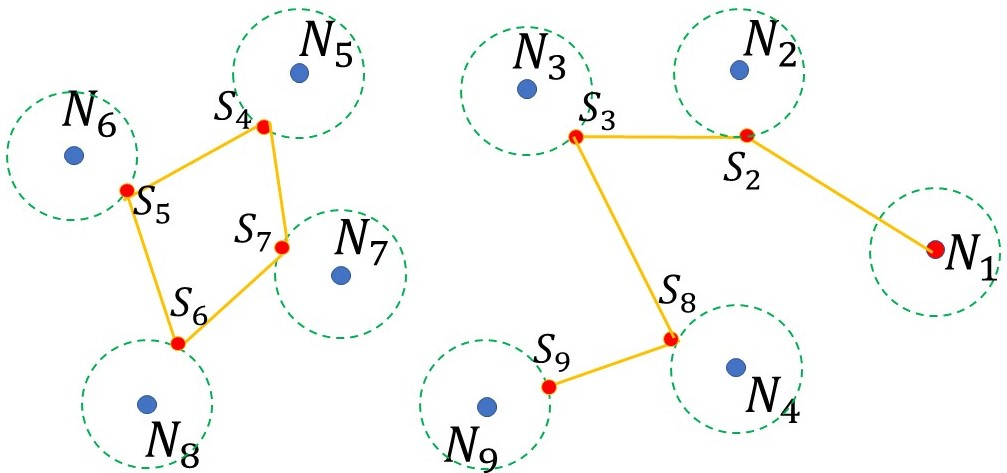
\includegraphics[height=1.4 true in]{DisjointSubtour.jpg}}
  \caption{Disjoint sub-path example. 
  %$(N_1,N_9)=$ (start,goal) nodes.
  }
  \label{fig:subtour}
  \vskip -0.2 true in
\end{figure}
%% ----------------------------------- %%

\noindent {\bf Problem \boldmath{$\# 1$:}} The solution to the following optimization problem solves the symmetric distance {\em s-t-CPP}:\\
  \begin{equation}\label{eq:OptProblem}
    (\mathcal{S},\vec{\xi}) =  \argmin_{\mathcal{S},\vec{\xi}} \sum_{i=2}^n \xi_{1i}\ d(S_1,S_i)
             +\sum_{i=2,j> i}^n \xi_{ij} d(S_i,S_j)
  \end{equation}
subject to
\begin{eqnarray}
  && \sum_{j=2}^n \xi_{1j} = 1, \quad \quad \sum_{i=1}^{n-1}\ \xi_{in} = 1 \label{eq:edge} \\
  && \sum_{j=1}^{i-1} \xi_{ji} + \sum_{j=i+1}^n\ \xi_{ij} = 2, \ \ \ \forall i=2,\ldots,(n-1),
               \label{eq:node_constraint}\\
  && \sum_{i\in W,j\in W} \xi_{ij} \le |W|-1, \ \forall W\in \mathcal{S} \backslash \{S_1,S_N\}, |W|\ge 3,
       \ \ \          \label{eq:subtour}\\
  && N_i\ \in R(S_i), \label{eq:inrange}\\
  &&  \xi_{ij}\ \in \ \{0,1\}, \label{eq:binary}
\end{eqnarray}
where the sensing range constraint (\ref{eq:inrange}) takes the form of Eq. (\ref{eq:quadratic}) or (\ref{eq:polytope}), or a convex combination of such constraints.

%% ------------------------------------------------------ %%
\subsection{Implementation Details and Example}

\noindent Problem $\# 1$ is a mixed integer nonlinear programming (MINLP) problem.  It is NP-hard \cite{current_efficient_1994}, since the CPP includes the $NP$-hard traveling salesman problem (TSP) as a special case (as $r_{max}\rightarrow 0$, the CPP becomes the TSP).  While MINLP solvers do not scale well,  they can tackle modest problems. The example in Fig. \ref{fig:MINLP_example} uses BONMIN \cite{BONMIN}, a branch-and-bound and a nonlinear trust region optimizer that produces globally optimal solutions.  BONMIN requires a problem seed.  Fig. \ref{fig:MINLP_example}(a), shows an intuitively poor initial guess.  The path in Fig. \ref{fig:MINLP_example}(b) was computed in 5.8 seconds\footnote{All evaluations use MATLAB 19a, the MATLAB Opti ToolBox\cite{OptiToolbox} with the BONMIN solver, and an Intel i7-4770 CPU with 16 Gbyte memory.}.

%% ----------------------------------- %%
\begin{figure}[h]
  \vskip -0.1 true in
\centerline{   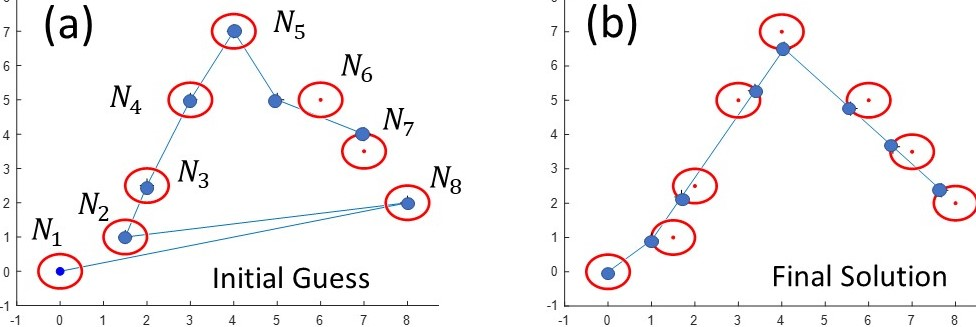
\includegraphics[height=1.0 true in]{BONMIN_Examples.jpg} }
  \caption{MINLP solution using BONMIN. (a) Initial path guess; (b) Optimal path.  The targets lie at the centers of the red circles, whose radii are the sensing range.  In a successful tour, each sensing node (blue dots) must lie in a circles.}
  \label{fig:MINLP_example}
  \vskip -0.15 true in
\end{figure}
%% ----------------------------------- %%

%%% ------------------------------------------------------------------------- %%
\section{A Polynomial Time Approximation with Bounded Approximation Ratio}\label{sec:polynomial}

\noindent This section introduces a 2-step approximation algorithm that produces a close to optimal path with computational complexity that is {\em polynomial} in $n$.  The first step finds and fixes a target node {\em path order}--the sequence to visit the targets.  Using this fixed order, the second step optimizes the sensing locations using an efficient quadratic program.  Subsequent sections extend this foundation. The visitation order is found using a small variation of {\em Hoogeven's algorithm} \cite{hoogeveen_analysis_1991}.\vspace{-3pt}

\subsection{The Hoogeeveen Approximation} \label{sec:Hoogeveen}

\noindent Hoogeveen's \cite{hoogeveen_analysis_1991} algorithm (Algorithm \ref{alg:hoogeveen}) generates a path for the {\em s-t-TSP} with a 5/3 approximation ratio (i.e., the path is no more than 5/3 times the optimal path length).  In Line \ref{line:MaxCompleteGraph}, the maximally complete weighted graph, $\mathcal{C}_{max}$, is constructed (in time $\Os(n^2)$) by joining every pair of target nodes, except $(N_1,N_n)$, with an undirected edge whose weight is $d(N_i,N_j)$.  Infeasible edges are removed.  Lines \ref{line:MST}-\ref{line:MPM} produce a graph whose structure can be further refined into an s-t-TSP path.  In Line \ref{line:Tjoin}, nodes $N_1$ and $N_n$ have the {\em wrong degree} if their degree in the
Minimum Spanning Tree is even, while nodes $\{N_2,\ldots,N_{n-1}\}$ have the ``wrong'' degree if their degree is odd.  These ``wrong'' degree nodes form a {\em T-join} of the minimum spanning tree $T_{MS}$ \cite{gao_metric_2018}. The minimum perfect matching of the T-join in Line \ref{line:MPM} can be found using
Blossom's algorithm \cite{kolmogorov_blossom_2009}, which requires $\mathcal{O}(n^3)$ computation. Lines \ref{line:EulerianTour} and \ref{line:Hamiltonian} convert and prune this intermediate graph (in time $\Os(n^3)$) to an admissible s-t-TSP path ($\Ps$ passes once through each node on the path graph), with a guaranteed path length no longer than $5/3$ times the optimal {\em s-t-TSP} solution.
%
%%% -------------------------------------------------------------- %%%
\begin{algorithm}[htb]
\caption{Hoogeveen s-t-TSP Heuristic}
\begin{small}
\begin{algorithmic}[1]
\Procedure{HoogeveenHeuristic}{$\mathcal{N}$ = target node set}
\State $\mathcal{C}_{max}\ =\ {\rm MaxCompleteWeightedGraph}(\mathcal{N})$ \label{line:MaxCompleteGraph}
\State $T_{MS}\ =\ {\rm MinSpanningTree}(\mathcal{C}_{max})$ \label{line:MST}
\State $T_{join}\ =\ {\rm WrongNodeDegree}(T_{MS})$ \label{line:Tjoin}
\State $T_{MPM}\ =\ {\rm MinPerfectMatching}(T_{join})$ \label{line:MPM}
\State $T_{union} = T_{MPM} + T_{MS}$    \label{line:union}
\State $T_{E}\ =\ {\rm EulerianTour}(T_{union})$ \label{line:EulerianTour}
\State $T_H\ =\ {\rm HamiltonianShortCut}(T_{E})$ \label{line:Hamiltonian}
\State ${\rm Return}(T_H)$.
\EndProcedure
\end{algorithmic}
\end{small}
\label{alg:hoogeveen}
\end{algorithm}
%%% -------------------------------------------------------------- %%%
%
\vskip -0.2 true in
\subsection{Efficient Optimization of Sensing Locations}

\noindent Alg. \ref{alg:hoogeveen} yields an efficient path that passes through the targets, but does not optimize the sensing locations.  If the sensing regions are not ``large'' (large sensing regions are analyzed in Section \ref{sec:fewer}), the path order found by Alg. \ref{alg:hoogeveen} is a good solution for the next step that optimizes the sensing locations.  A given path ordering fixes the incidence variables, $\{\xi_{ij}\}$, reducing cost (\ref{eq:min_cost}) to be quadratic. Thus, optimization of sensing node locations is an efficient quadratic program with quadratic or linear constraints \cite{boyd}, depending on the type of sensor.  These concepts are summarized in Alg. \ref{alg:s_t_heuristic}.
%
%%% -------------------------------------------------------------- %%%
% \setlength{\textfloatsep}{5pt}
\begin{algorithm}[t]
\caption{s-t-CPP Approximation}
\begin{small}
\begin{algorithmic}[1]
\Procedure{s-t-Heuristic}{$\Ns$ = target node set}
\State $\mathcal{P}_{order}\ =\ {\rm HoogeveenHeuristic}(\mathcal{N})$
\State $\{\bar{\xi}_{ij}\}\ =\ {\rm Incidence}(P_{order})$ \label{line:getincidence}
\State $\mathcal{S}= \argmin {\rm Cost}(\bar{\xi},\mathcal{S},\mathcal{N})$ \label{line:argmin}
\State $\quad \quad {\rm subject\ to}\ N_i\ \in R(S_i)\ {\rm for}\ i=,2\ldots,n$ \label{line:SenseConstraint}
\State $\mathcal{P}_{h}\ =\ {\rm Path}(\mathcal{S},\bar{\xi})$ \label{line:path}.
\State ${\rm Return}(\mathcal{P}_h)$
\EndProcedure
\end{algorithmic}
\end{small}
\label{alg:s_t_heuristic}
\end{algorithm}

%%% ---------------------------------------------------- %%
{\bf Examples.} When Alg. \ref{alg:s_t_heuristic} is applied to the problem of Fig. \ref{fig:MINLP_example}, it yields the same solution in 0.1 sec.  Note that Alg. \ref{alg:s_t_heuristic} {\em does not} require a seed like the MINLP solution. Fig. \ref{fig:ManyDisjointNodes} shows an example with 18 targets placed at integer locations.  The path was found and optimized in ~0.25 seconds by Alg. \ref{alg:s_t_heuristic}.  The BONMIN MINLP solver could not solve this problem.
%
%% ------------------------------ %%
\begin{figure}[h]
\vskip -0.1 true in
    \centerline{
    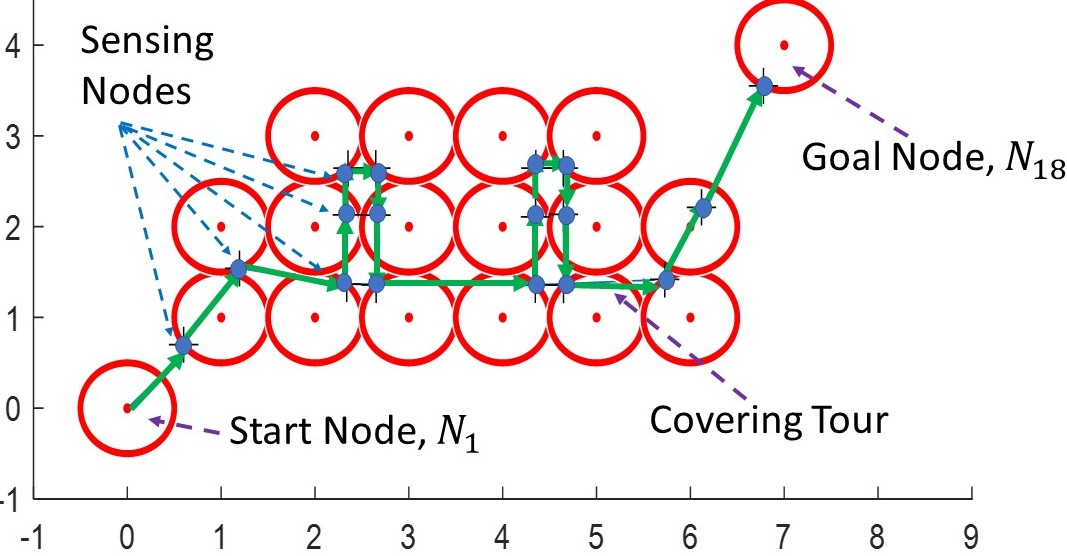
\includegraphics[height=1.5 true in]{ManyDisjointNodes.jpg}
    }
    \caption{Covering path calculated by Alg. \ref{alg:s_t_heuristic}.
      The 18 target are located in the centers of the red circles, whose radii equal the robot's sensing range.  The covering path is green, while the 18 blue dots indicate the sensing nodes.}
    \label{fig:ManyDisjointNodes}
    \vskip -0.2 true in
\end{figure}
%% ------------------------------ %%

%%% ---------------------------------------------------- %%
\subsection{A Bound on the Approximation Ratio}\label{sec:competitiveness}

\noindent Alg. \ref{alg:s_t_heuristic} has a {\em bounded} approximation ratio.  This result builds upon Hoogeveen's bound for the {\em s-t-TSP}  \cite{hoogeveen_analysis_1991}.

\begin{lemma}{\cite{hoogeveen_analysis_1991}} \label{lemma:hoogeveen} Given $n$ distinct targets $N_1,\ldots,N_n$, Alg. \ref{alg:hoogeveen} produces a path starting at $N_1$, passing through  $N_2,\ldots,N_{n-1}$ (not necessarily in that order), and ending at $N_n$.  The path length is no more than 5/3 of the  optimal {\em s-t-TSP} path length for the same problem.
\end{lemma}
%
\noindent Using this result, we have the following:
\begin{prop} \label{prop:bound1}
Consider $n>4$ target nodes which are all located at least twice the maximal sensing radius, $r_{max}$, from each other.  Alg. \ref{alg:s_t_heuristic} produces a valid s-t covering path, $\mathcal{P}_h$, of the $n$ targets. For $n$ odd, the length of covering path, $|\mathcal{P}_h|$, is bounded relative to the length of optimal covering path $|\mathcal{P}^*|$ as
   \begin{equation}\label{eq:bound_odd}
      |\mathcal{P}^{odd}_h| \ \le \ \frac{10(n-1)}{3(n-4+\sqrt{5-2\sqrt{3}})}|\mathcal{P}^*|\ ,
   \end{equation}
   and for $n$ even the path length is bounded as
   \begin{equation}\label{eq:bound_even}
      |\mathcal{P}^{even}_h| \ \le \ \frac{10(n-1)}{3(n-4+ 2\sqrt{3})}|\mathcal{P}^*|\ .
   \end{equation}
Moreover, $|\mathcal{P}_h|$ is computed in time proportional $\mathcal{O}(n^4)$.
\end{prop}

For large $n$, the approximation ratio ${\Rs_{app}}$ is bounded by $10/3$, which is better than the best ratios in \cite{de_berg_tsp_2005,Mitchel}}.

\vskip 0.07 true in
\noindent {\bf Proof Sketch:}  A bound on $\Rs_{app}$, is computed as follows:
  \begin{equation} \label{eq:comp1}
      \Rs_{app} = \frac{L_h}{L^{*}_{CPP}} \ \le \  \frac{\bar{L}_h}{\underbar{\em L}^{*}_{CPP}}
  \end{equation}
where $L_h$ is the path length produced by Alg. \ref{alg:s_t_heuristic}, and $\bar{L}_h$ is an {\em upper bound} on that length.  Similarly, $\underbar{\em L}^{*}_{CPP}$ is a {\em lower bound} on the optimal covering path length, $L^{*}_{CPP}$.  The CPP path produced by Alg. \ref{alg:s_t_heuristic} is a
reduction of the TSP solution found in Alg. \ref{alg:hoogeveen}, and cannot be longer than the approximation ratio of Lemma \ref{lemma:hoogeveen}: 
$(5/3)L^{*}_{TSP}$.  Thus, $\bar{L}_h\le (5/3)L^{*}_{TSP}$.
%
%% ------------------------------ %%
\begin{figure}[htb]
  \vskip -0.1 true in
  \centerline{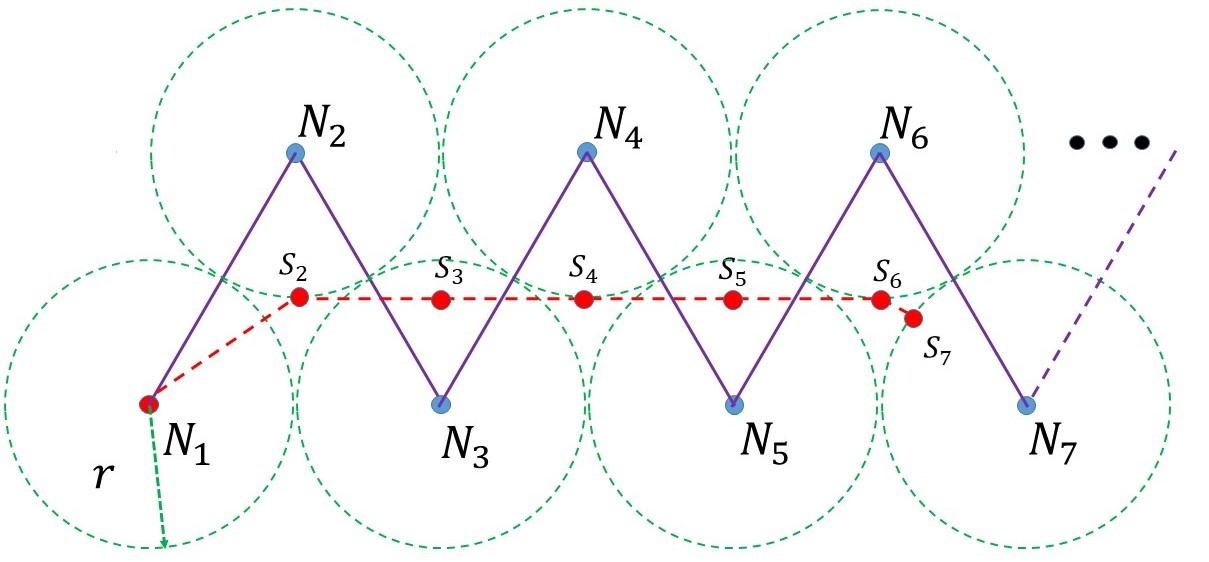
\includegraphics[height=1.2 true in]{CompetitivenessDiagram.jpg}}
    \caption{Geometry of worst case ratio of $L^{*}_{TSP}$ to $L^*_{CPP}$}
    \label{fig:CompetitivenessDiagram}
    \vskip -0.1 true in
\end{figure}
%% ------------------------------ %%

To develop an expression for $\underbar{\em L}^{*}_{CPP}$, consider the covering problem in Fig. \ref{fig:CompetitivenessDiagram}. The circles depict the maximum sensing range centered on the targets.  These barely touching circles are nested in an alternating linear pattern.  It can be shown that this geometry leads to the shortest covering path, relative to the TSP path that visits all targets, for all problem geometries.  For odd numbers of nodes, $L^{*}_{CPP} = (n-4 + 2 \sqrt{5-2\sqrt{3}})r$. Since the TSP path length is $2(n-1)r$, the optimal CPP path length is lower bounded by the ratio of these path lengths times $L^{*}_{TSP}$: $\underbar{\em L}^{*}_{CPP} = \frac{(n-4 + \sqrt{5-2\sqrt{3}})}{2(n-1)} L^{*}_{TSP}$.  Substituting $\underbar{\em L}^{*}_{CPP}$ and $\bar{L}_{h}$ into Eq. (\ref{eq:comp1}), and dividing through by $L^{*}_{TSP}$ yields Eq. (\ref{eq:bound_odd}).  When $n$ is even,  $L^{*}_{CPP}=(n-4 + 2\sqrt{3})r$, while $L^{*}_{TSP}=2(n-1)r$.  Substituting these results into (\ref{eq:comp1}) yields Eq. (\ref{eq:bound_odd})

Algorithm correctness follows from construction.  No step in Alg. \ref{alg:hoogeveen} has complexity greater than $\Os(n^3)$. Complexity is dominated by the $\Os(n^4)$ optimization in Alg. \ref{alg:s_t_heuristic} $\qed$

%%% ------------------------------------------------------------------------------------------ %%
\section{Fewer Sensing Nodes than Target Nodes} \label{sec:fewer}

\noindent When target nodes are close together, a single sensing node may  cover multiple targets, potentially leading to shorter sensory coverage paths.  This section provides a formal statement of an optimization problem that finds these reductions. An algorithm to approximate this computationally difficult problem follows, and its properties are established.

Let $N_S\leq N$ denote the {\em variable} number of sensing nodes.
Since there may be fewer sensing nodes than target nodes, we must modify the sensing region constraint (\ref{eq:inrange}) in a subtle manner: for each target $N_i$ we require $||S_j - N_i|| \le r^2$ ($i=1,\ldots,N$) to be satisfied for {\em at least one} sensing node index, $j$.  This constraint can be expressed in disjunctive form:
   \[ \bigvee_{i=1}^{N_S} \big[ ||S_j - N_i||^2-r^2 \le 0 \big] .\]
Using a {\em Big-M} methodology \cite{vecchietti_modeling_2003}, this disjunction can be equivalently expressed as the set of mixed integer constraints (for each $i$) found in Eq.s (\ref{eq:bigM}), (\ref{eq:atleastone}), and (\ref{eq:etadefn}) below.  The constants $M_i$ must be chosen sufficiently large:
   \begin{equation} 
   M_i \ge \max_j\{ ||S_j-N_i||^2\ |\ S_j^{lower} \le S_j \le S_j^{upper}\}
   \end{equation}
where $S_j^{lower}$ and $S_j^{upper}$ are lower and upper bounds on $S_j$.  The binary variables $\{\eta_{ij}\}$ indicate sensing relationships: $\eta_{ij}=1$ if $N_i\ \in \ R(S_j)$, else $\eta_{ij}=0$.

{\bf Problem \boldmath{$\# 2$}:} The solution to the following optimization problem {\em exactly} solves the {\em s-t-CPP} when $N_S\le N$:\\
  \begin{equation}\label{eq:OptProblemFull}
    (N_S,\mathcal{S},\vec{\xi}) \!= \! \argmin_{N_S,\mathcal{S},\vec{\xi}} \
            \sum_{i=2}^{N_S} \xi_{1i}d(S_1,S_i)
             + \!\!\sum_{j=i,j\ne i}^{N_S} \! \!\xi_{ij} d(S_i,S_j)
  \end{equation}
subject to Eqs (\ref{eq:edge}), (\ref{eq:node_constraint}), (\ref{eq:subtour}), (\ref{eq:binary}), and $\forall i=1,\ldots,n$:
\begin{eqnarray}
    && ||S_j - N_i|| \le r^2 + (1-\eta_{ij}) \cdot M_i \ \ \forall j=1,\ldots,N_S   \label{eq:bigM}\\
    && \sum_{j=1}^{N_S} \ \eta_{ij} \ge 1 \ \  \ \forall j=1,\ldots,N_S  \label{eq:atleastone} \\
    && \eta_{ij}\ \in \ \{0,1\}  \ \ \ \forall j=1,\ldots,N_S\ .  \label{eq:etadefn}
\end{eqnarray}
Eq. (\ref{eq:atleastone}) ensures that one sensing node covers each target.

To our knowledge, this formulation represents the first complete statement of the {\em s-t-CPP} problem with the option of variable numbers of sensing nodes.

\setlength{\textfloatsep}{15.0pt plus 2.0pt minus 2.0pt}

\subsection{An Approximation Algorithm for Variable Sensing Nodes} \label{sec:overlap_heuristic}

\noindent Problem $\# 2$ forms an additionally constrained version of the NP-hard Problem $\# 1$.  The simple heuristic described in this section takes advantage of opportunities to reduce the number of sensing nodes. Its properties are analyzed below.\vspace{-11pt}
%
%% ------------------------------ %%
\begin{figure}
  \centerline{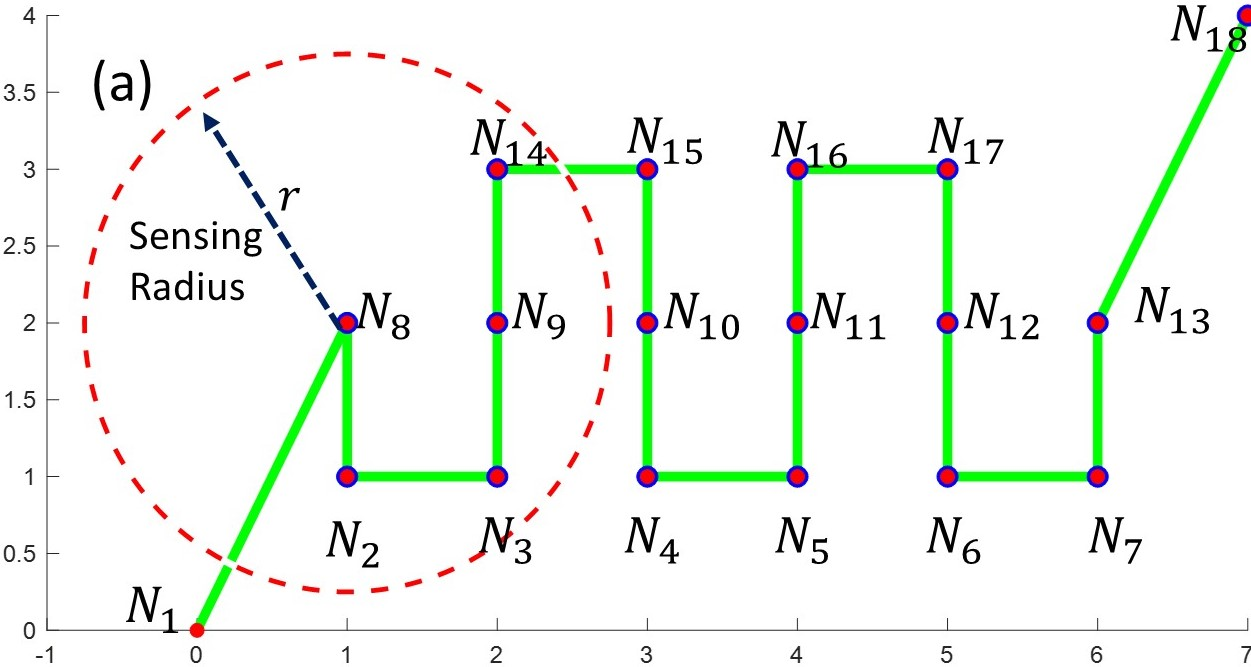
\includegraphics[height=1.2 true in]{Overlap18a.jpg}}
  \centerline{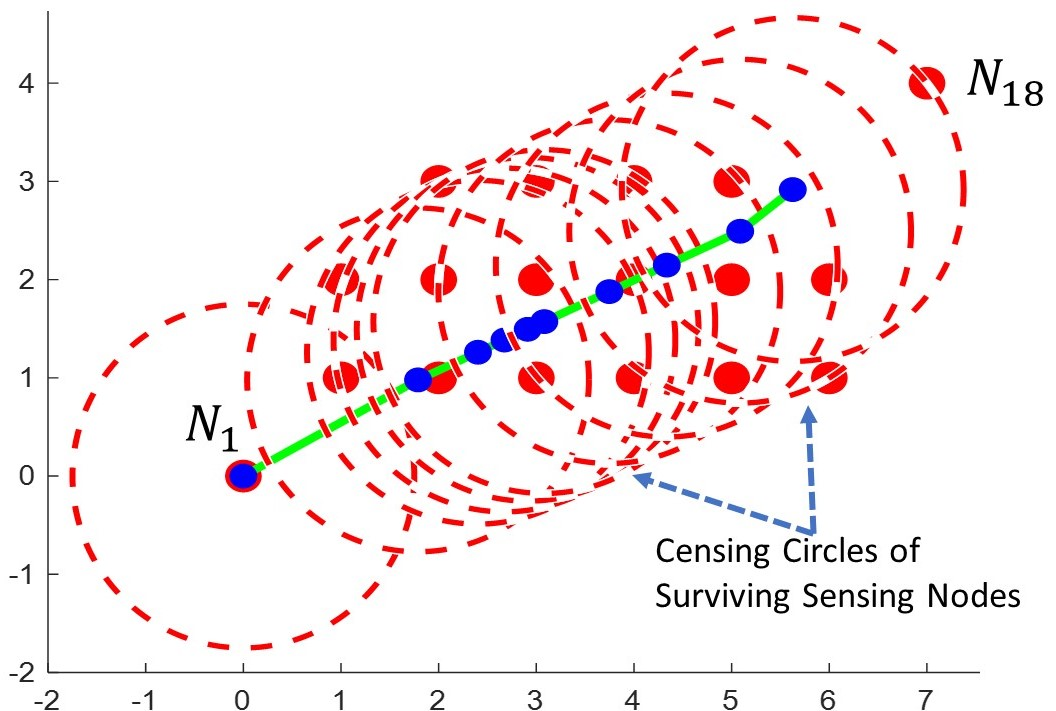
\includegraphics[height=1.4 true in]{Overlap18b.jpg}}
    \vskip -0.05 true in
  \caption{An 18 Target (red dots) problem. The dashed red circles depicts the robot's sensing range. (a) The green path results from applying  Alg. \ref{alg:hoogeveen} to the targets.  (b) The result of applying  Alg. \ref{alg:s_t_heuristic} to optimize the sensing  locations (blue dots). The sensing circles of  10 surviving sense nodes are shown.}
  \label{fig:overlap1}
  \vskip -0.1 true in
\end{figure}
%% ------------------------------ %%

Fig. \ref{fig:overlap1} shows the 18 target example of Fig. \ref{fig:ManyDisjointNodes}, but with a larger sensing range ($r=1.75$ units), which allows one sensing node to cover multiple targets.  Fig. \ref{fig:overlap1}(a) shows the path resulting from Alg. \ref{alg:hoogeveen}. Note that Alg. \ref{alg:hoogeveen} often produces {\em boustrophedan-like} \cite{choset_coverage_2000} paths when applied to problems with repeating geometries. In Fig. \ref{fig:overlap1}(b) Alg. \ref{alg:s_t_heuristic} has optimized the sensing locations based on the Fig. \ref{fig:overlap1}(a) path order.

Many sensor nodes can be eliminated, without reducing coverage. The problem of eliminating unnecessary sensing nodes is equivalent to the $NP$-hard {\em Bin Packing} or {\em Set-Cover} problems \cite{du_applications_1998,approx_alg}.  Hence, practically useful pruning methods must be a polynomial complexity approximations. Ou demonstrations use a simple algorithm, SensingNodeReduction($\Ss$),  that starts at $S_{N_S}$ and progresses backward along the path, removing sensing nodes whose targets are covered by other sensors.  This $\Os(n^2)$ process is one of many possible pruning algorithms. When Alg. \ref{alg:overlap_reduce} is applied to the sensing node path  of Fig. \ref{fig:overlap1}(b), 8 sensing nodes are removed. The large blue dots in Fig. \ref{fig:overlap1}(b) are the surviving sensing nodes.  An optimal analysis of this problem allows 12 nodes to be removed.
%
%%% -------------------------------------------------------------- %%%
%\vspace{-2mm}
%\begin{algorithm}[htb]
%\caption{Overlap Pruning Heuristic}
%\begin{small}
%\begin{algorithmic}[1]
%  \Procedure{SensingNodeReduction}{$\Ss$}
%\State{DoNotRemove = []}
%\For{$i=n$ down to $2$}    \label{line:candidate}
%\For{$j=i-1$ down to $1$, $j\ne i$}
%\If{$(S_i\ \in\ R(S_j))$ and ($S_i\notin$ DoNotRemove)}
%\State{Remove Node $S_i$; \ \ Add $S_j$ to DoNotRemove} 
%\State{Add edge $(S_{i-1},S_{i+1})$ if $S_{i+1}$ exists}
%\State{Break}
%\EndIf
%\EndFor 
%\EndFor
%\State{Return $\Ss$}
%\EndProcedure
%\end{algorithmic}
%\end{small}
%\label{alg:overlap}
%\end{algorithm}
%\vspace{-4mm}

%%% -------------------------------------------------------------- %%%
\vskip -0.25 true 
%%% -------------------------------------------------------------- %%%
% \vspace{-2mm}
\begin{algorithm}[ht]
\caption{Multi-Target Covering Heuristic}
\begin{small}
\begin{algorithmic}[1]
\Procedure{ReducedSensingPath}{$\{\Ns\}$}
\State{$\Ss$ = s-t-Heuristic($\Ns$)}
\State{$\Ss^{'}$ = SensingNodeReduction($\Ss$)}
\State{Return $\Ss^{'}$}
\EndProcedure
\end{algorithmic}
\end{small}
\label{alg:overlap_reduce}
\end{algorithm}
% \vspace{-2mm}
%%% -------------------------------------------------------------- %%%

\subsection{Performance Analysis}

\noindent Any approximation ratio for Alg. \ref{alg:s_t_heuristic} {\em must} depend upon the sensing range, $r$.  When $r$ is small, we recover the ratio of Prop. \ref{prop:bound1}.  However, as $r\rightarrow \infty$, the robot need not move to view all targets (ignoring occluding obstacles).  In that case, the denominator of $\Rs_{app}$ in Eq. (\ref{eq:comp1}), $L^{*}_{CPP}$, is $0$.  Since $\Rs_{app}$ is not well defined in this case, there are no meaningful approximation bounds for Alg.  \ref{alg:overlap_reduce}. However, Prop. \ref{prop:bound_overlap} provides a practical characterization of Alg. \ref{alg:overlap_reduce}.

\begin{prop} \label{prop:bound_overlap}
Given $n$ targets, with subgroupings that can each be covered by a single sensor node, Alg. \ref{alg:overlap_reduce} constructs a covering path in $\Os(n^4)$ time with $N_S\le (n-1)$.  The path length is bounded by $(5/3)L_{TSP}(\Ns)-r$, where $L_{TSP}(\Ns)$ is the optimal traveling salesman path length over the targets.
\end{prop}

\noindent {\bf Proof sketch:} Because Alg. \ref{alg:overlap} is $\Os(n^2)$, Alg. \ref{alg:overlap_reduce} inherits the $\Os(n^4)$ complexity from Prop. \ref{prop:bound1}.  Alg. \ref{alg:overlap} will remove at least one unneeded sensing node when sensing overlaps exist.  The bound on path length is derived from Lemma \ref{lemma:hoogeveen}.

%%% ------------------------------------------------------------------------- %%
\section{Complete Sensory Coverage}\label{sec:complete_coverage}

\noindent This section extends our covering path framework to the {\em complete sensory coverage} problem, where all points in a bounded freespace, $\Ws$, must be covered by the robot's sensors.  We assume that $\Ws$'s outer boundary is polygonal, and allow for an arbitrary number of (possibly non-convex) interior polygonal obstacles.  $\mathcal{W}$ can partitioned into $N_{cell}$ disjoint convex polygons, $\{\Cs_i\}$, $i=1,\ldots,N_{cell}$, using for instance the {\em Voronoi diagram} of $\Ws$. %%$\bigcup_{i=1}^{N_{cell}} \Cs_i = \mathcal{W}$ and $\Cs_i \bigcap %\Cs_j=\emptyset$ $\forall i\ne j$.  
This is the advantage of an optimization-based formulation: the cells need not have the same size or number of vertices. We only require that the robot's sensor can cover the largest cell.  
%
%% ------------------------------ %%
\begin{figure}
  \vskip -0.05 true in
  \centerline{
  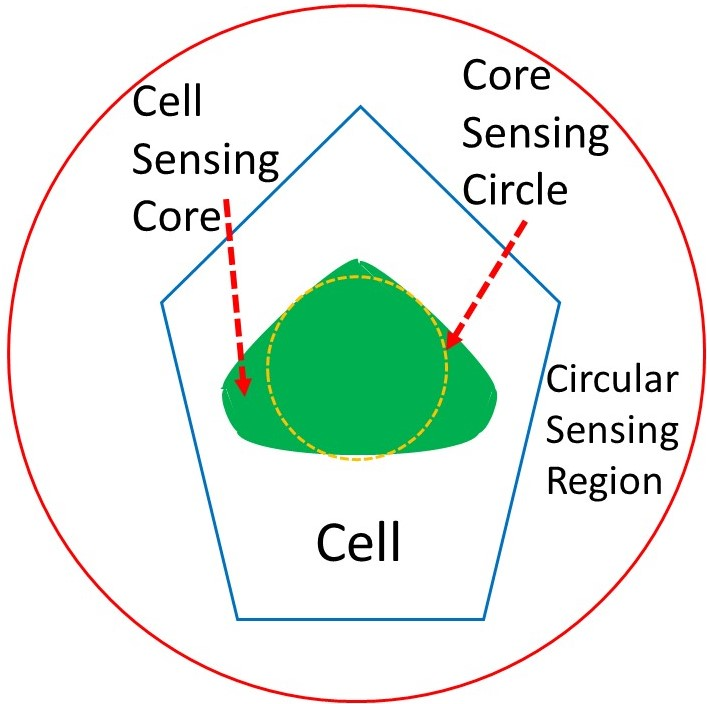
\includegraphics[height=1.0 true in]{CellSensingCore.jpg}
  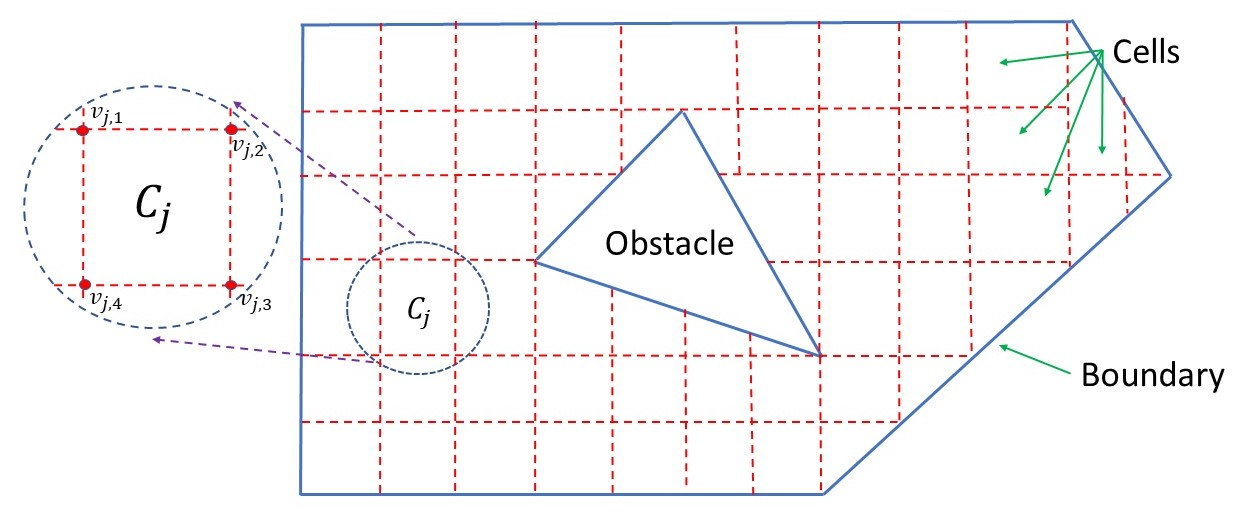
\includegraphics[height=1.0 true in]{FreespaceDivision.jpg}
  }
      \vskip -0.05 true in
  \caption{(a) Cell Sensing Core diagram; (b) Disjoint decomposition of freespace into non-uniform convex cells.  A cell $\mathcal{C}_j$ (circular inset), is defined by vertices $v_{j,1},\ldots,v_{j,p_j}$.}
  \label{fig:completecoverage}
    \vskip -0.2 true in
\end{figure}
%% ------------------------------ %%

Cell $\mathcal{C}_i$ is {\em covered} by the robot's sensors at position $S_j$ if $\mathcal{C}_i\ \subseteq\ R(S_j)$.  To completely cover $\mathcal{W}$,  each cell must be covered by at least one sensing node.  We can represent this complete coverage condition as: $ \bigvee_{j=1}^{N_S}\ \big[\cell_i \ \subseteq\ R(S_j)\big] \ \forall i=1,\ldots,N_{cell}$.  To convert this condition into a computation, recall that the sensing pattern is a convex set.  Convex cell $\Cs_i$ will be covered at location $\Ss_j$ if all of its vertices, $\{v_{i,1},\ldots,v_{i,p_i}\}$, lie inside $R(S_j)$. For a circular sensing region with radius $r$, this constraint can be expressed as 
   \begin{equation}\label{eq:complete2}
    \bigvee_{j=1}^{N_S}\ \big[\wedge_{k=1}^{p_k} (v_{i,k}-S_j)^2\le r^2\big]\ \ \  \forall i=1,\ldots,N_{cell}\ .
  \end{equation}
Using distributive laws and the {\em Big-M} framework, constraint (\ref{eq:complete2}) can be expressed as $N_S \cdot N_{cell} \cdot \sum_{i=1}^{N_{cell}} p_i$ mixed integer constraints (\ref{eq:NewbigM}) and (\ref{eq:etadefn}), with $N_{cell}$ linear constraints (\ref{eq:Newatleastone}) on the binary variables $\eta_{ij}$.  The variables $\eta_{ij}$ have an analogous meaning to Eq. (\ref{eq:etadefn}): $\eta_{ij}=1$ if the robot's sensors completely cover $\cell_i$ when the robot lies as position $S_j$.

{\bf Problem \boldmath{$\# 3$}:} Assume that the freespace of a polygonal workspace (with polygonal obstacles) can be decomposed into convex polygonal cells. If the robot's sensors can cover the largest individual cell, the shortest complete sensory coverage path is the solution to the following:
  \begin{equation}\label{eq:OptProblemFull}
    (N_S,\mathcal{S},\vec{\xi}) =  \argmin_{N_S,\mathcal{S},\vec{\xi}} \
            \sum_{i=2}^{N_S} \xi_{1i}d(S_1,S_i)
             + \sum_{j=i,j\ne i}^{N_S} \xi_{ij} d(S_i,S_j)
  \end{equation}
subject to Eq.s (\ref{eq:edge}), (\ref{eq:node_constraint}), (\ref{eq:subtour}), (\ref{eq:binary}), (\ref{eq:etadefn}), and $\forall i=1,\ldots,N_{cell}, \  \forall j=1,\ldots,N_S$:
\begin{eqnarray}
    ||S_j - v_{i,1}||^2  & \le & r^2 + M_{ij}(1-\eta_{ij}) \nonumber \\
                       & \vdots &  \label{eq:NewbigM}\\
    ||S_j - v_{i,p_i}||^2 & \le & r^2 - M_{ij}(1-\eta_{ij}) \nonumber\\
\sum_{j=1}^{N_S}\ \eta_{ij} & \ge & 1 \ \ \ \ \forall i=1,\ldots, N_{cell}  \label{eq:Newatleastone} 
\end{eqnarray}

\subsection{A Complete Coverage Approximation Algorithm}

\noindent An approximate solution to Problem $\# 3$  requires only a small change to the previous heuristics, because cells are the input.  Let $\Cs^g_i = (1/p_i) \Sum_{j=1}^{p_i}v_{ij} $ denote the geometric center of cell $\Cs_i$. Alg. \ref{alg:sensory_coverage} follows the 2-step approximation scheme used above. Alg. \ref{alg:s_t_heuristic} is applied (Line \ref{line:Sensory-s-t}) to the cell centers (computed in Line \ref{line:centers}).  Alg. \ref{alg:s_t_heuristic} first fixes a cell visitation order by applying Alg. \ref{alg:hoogeveen} to the cell centers.  Then, the sensing locations are optimized (Alg. \ref{alg:s_t_heuristic}, Lines \ref{line:argmin}, \ref{line:SenseConstraint}).  However, in Line \ref{line:SenseConstraint} of Alg. \ref{alg:s_t_heuristic}, the condition $N_i\in R(S_i)$ must be replaced by $\Cs_i\subseteq R(S_i)$, which is condition (\ref{eq:complete2}), or equivalently Eq. (\ref{eq:NewbigM}) for the given $i$ and $j$. Finally, unneeded sensing nodes are removed in Line \ref{line:CompleteReduce}. Optionally, the reduced sensing node locations can be reoptimized (Alg. \ref{alg:s_t_heuristic}, Lines \ref{line:argmin}, \ref{line:SenseConstraint}).

%%% -------------------------------------------------------------- %%%
\vspace{-2mm}
\begin{algorithm}[htb]
\caption{Complete Sensory Coverage Approximation}
\begin{small}
\begin{algorithmic}[1]
\Procedure{SensoryCoverage}{$\{\Cs\}=$ cell definitions}
\State{$g$ = ComputeCellCenters($\{\Cs\}$)} \label{line:centers}
\State{$\Ss$ = S-T-Heuristic($g$)} \label{line:Sensory-s-t}
\State{$\Ss^{''}$ = SensingNodeReduction($\Ss^{'}$)}\label{line:CompleteReduce}
\State{Return $\Ss^{''}$}
\EndProcedure
\end{algorithmic}
\end{small}
\label{alg:sensory_coverage}
\end{algorithm}
\vspace{-3mm}
%%% -------------------------------------------------------------- %%%
%
%% ------------------------------ %%
\begin{figure}[h]
  \centerline{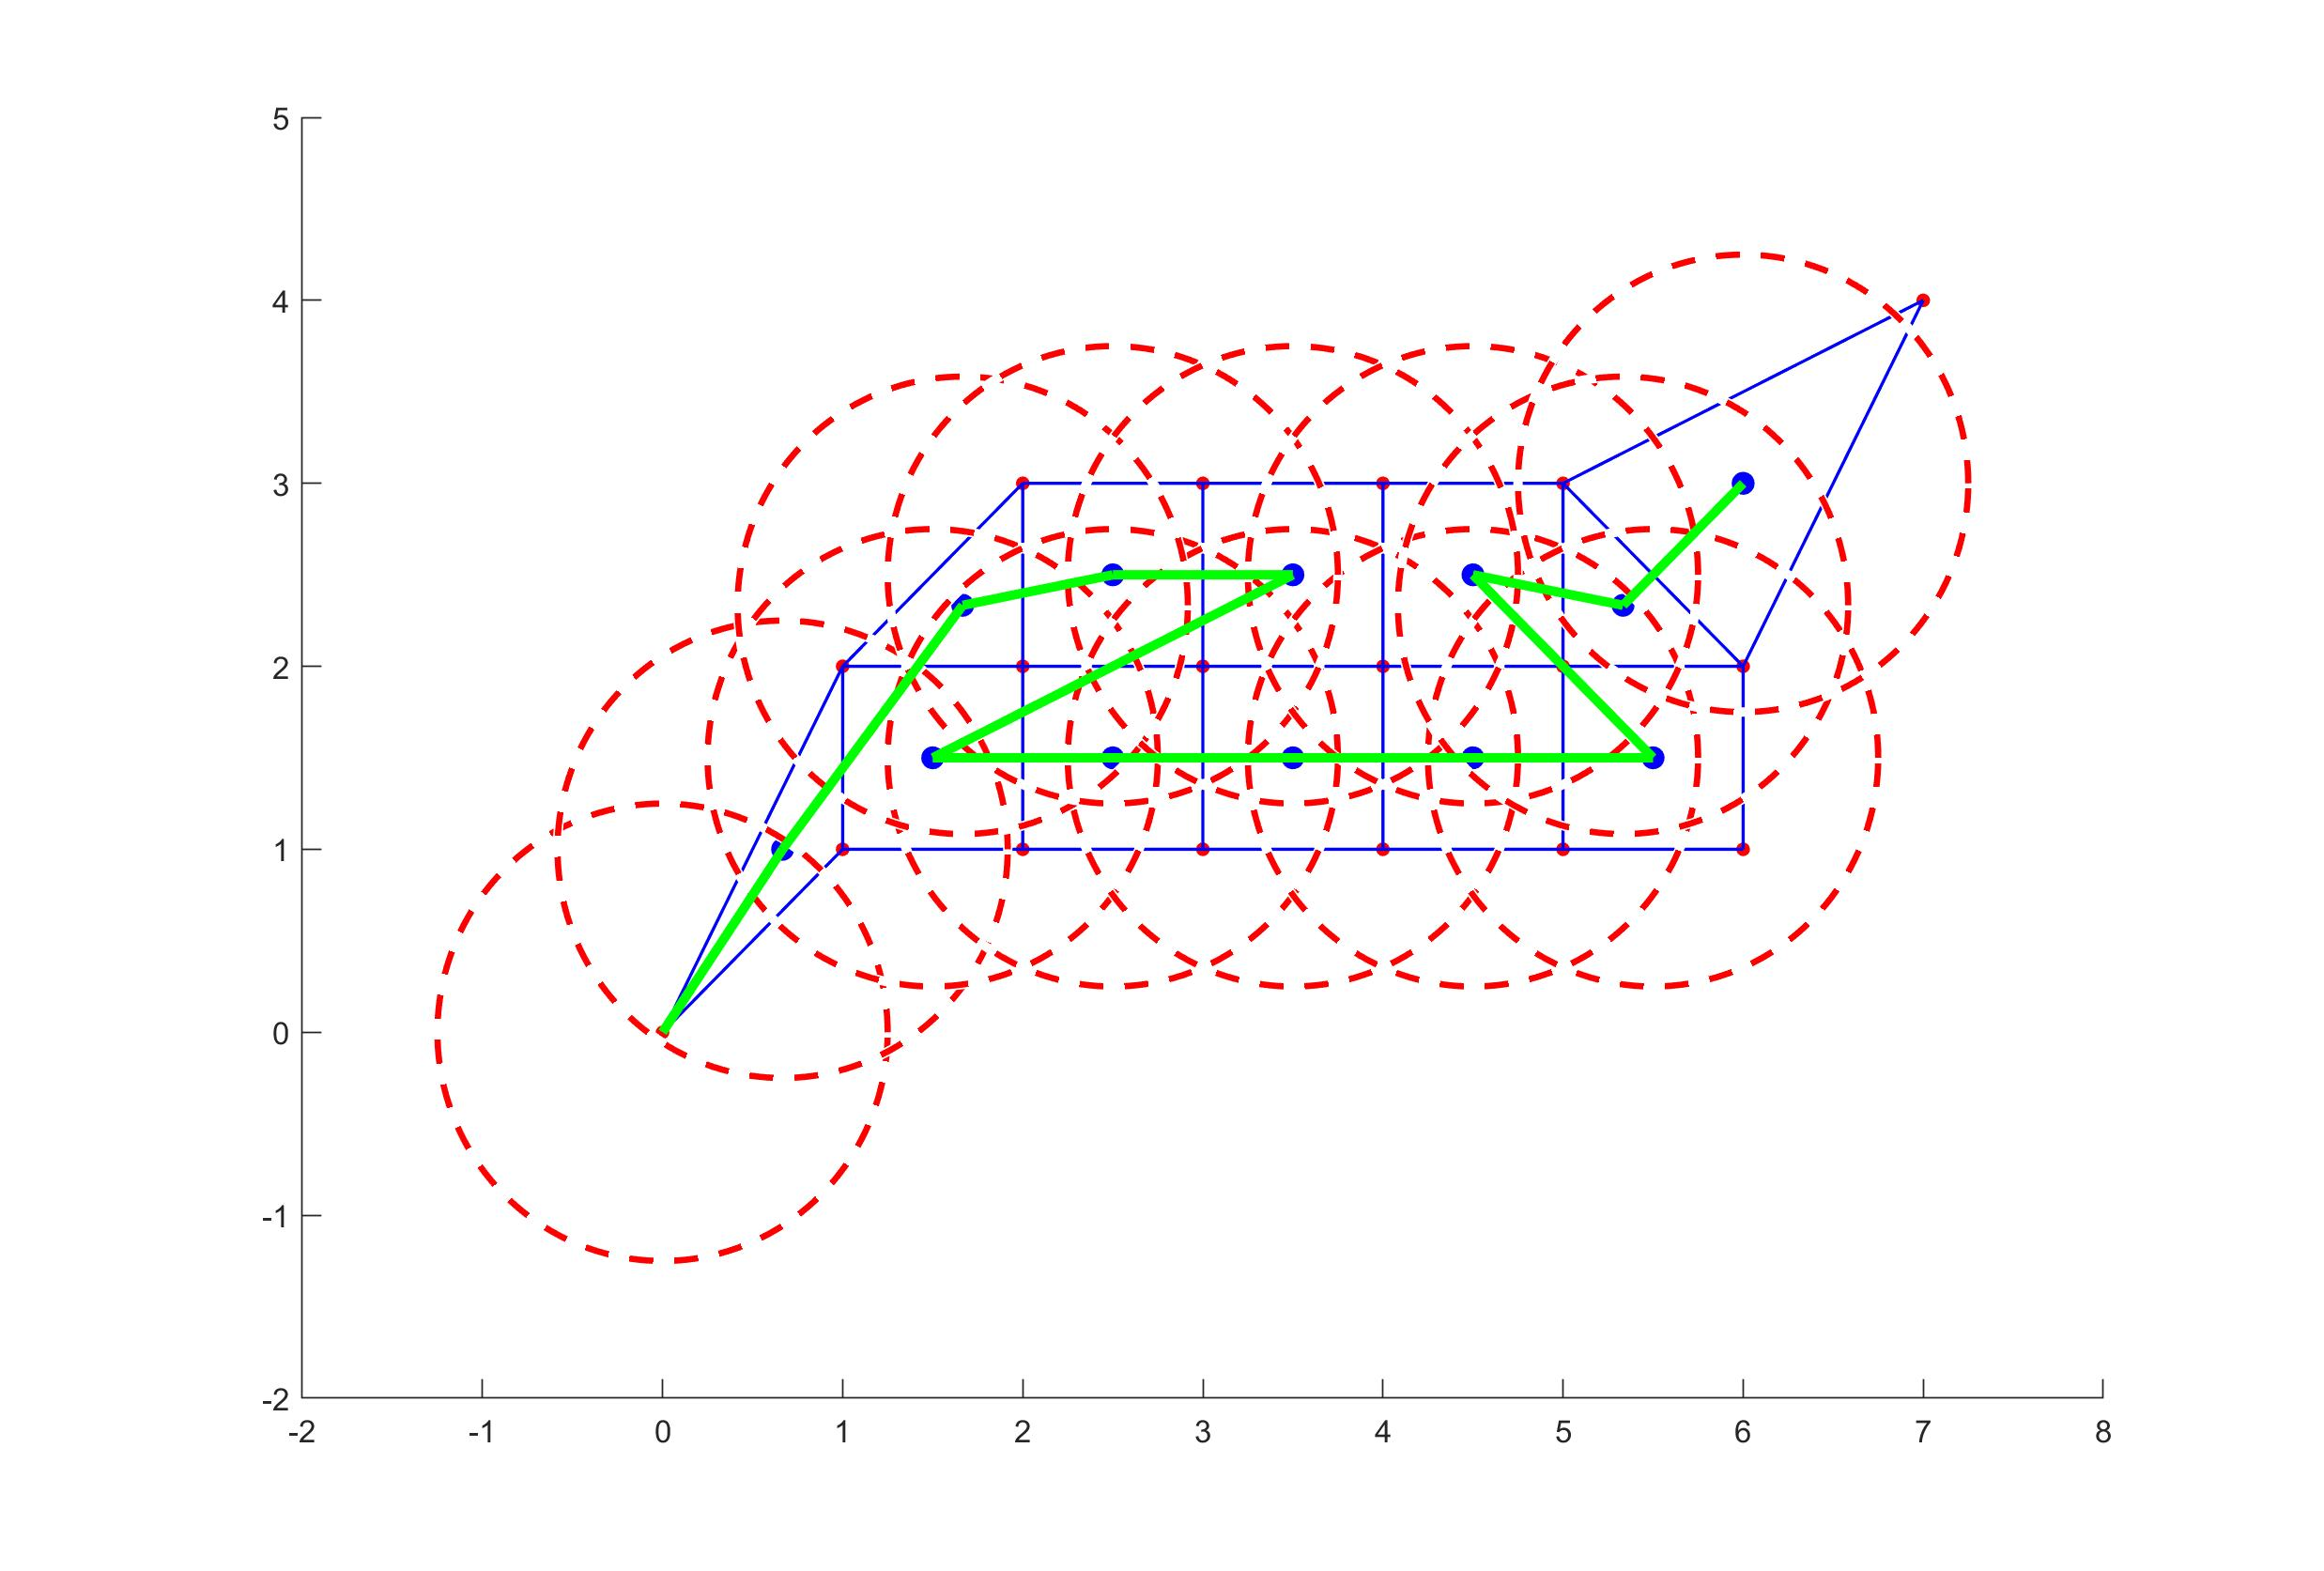
\includegraphics[height=1.6 true in]{Complete_Pre.jpg}}
  \centerline{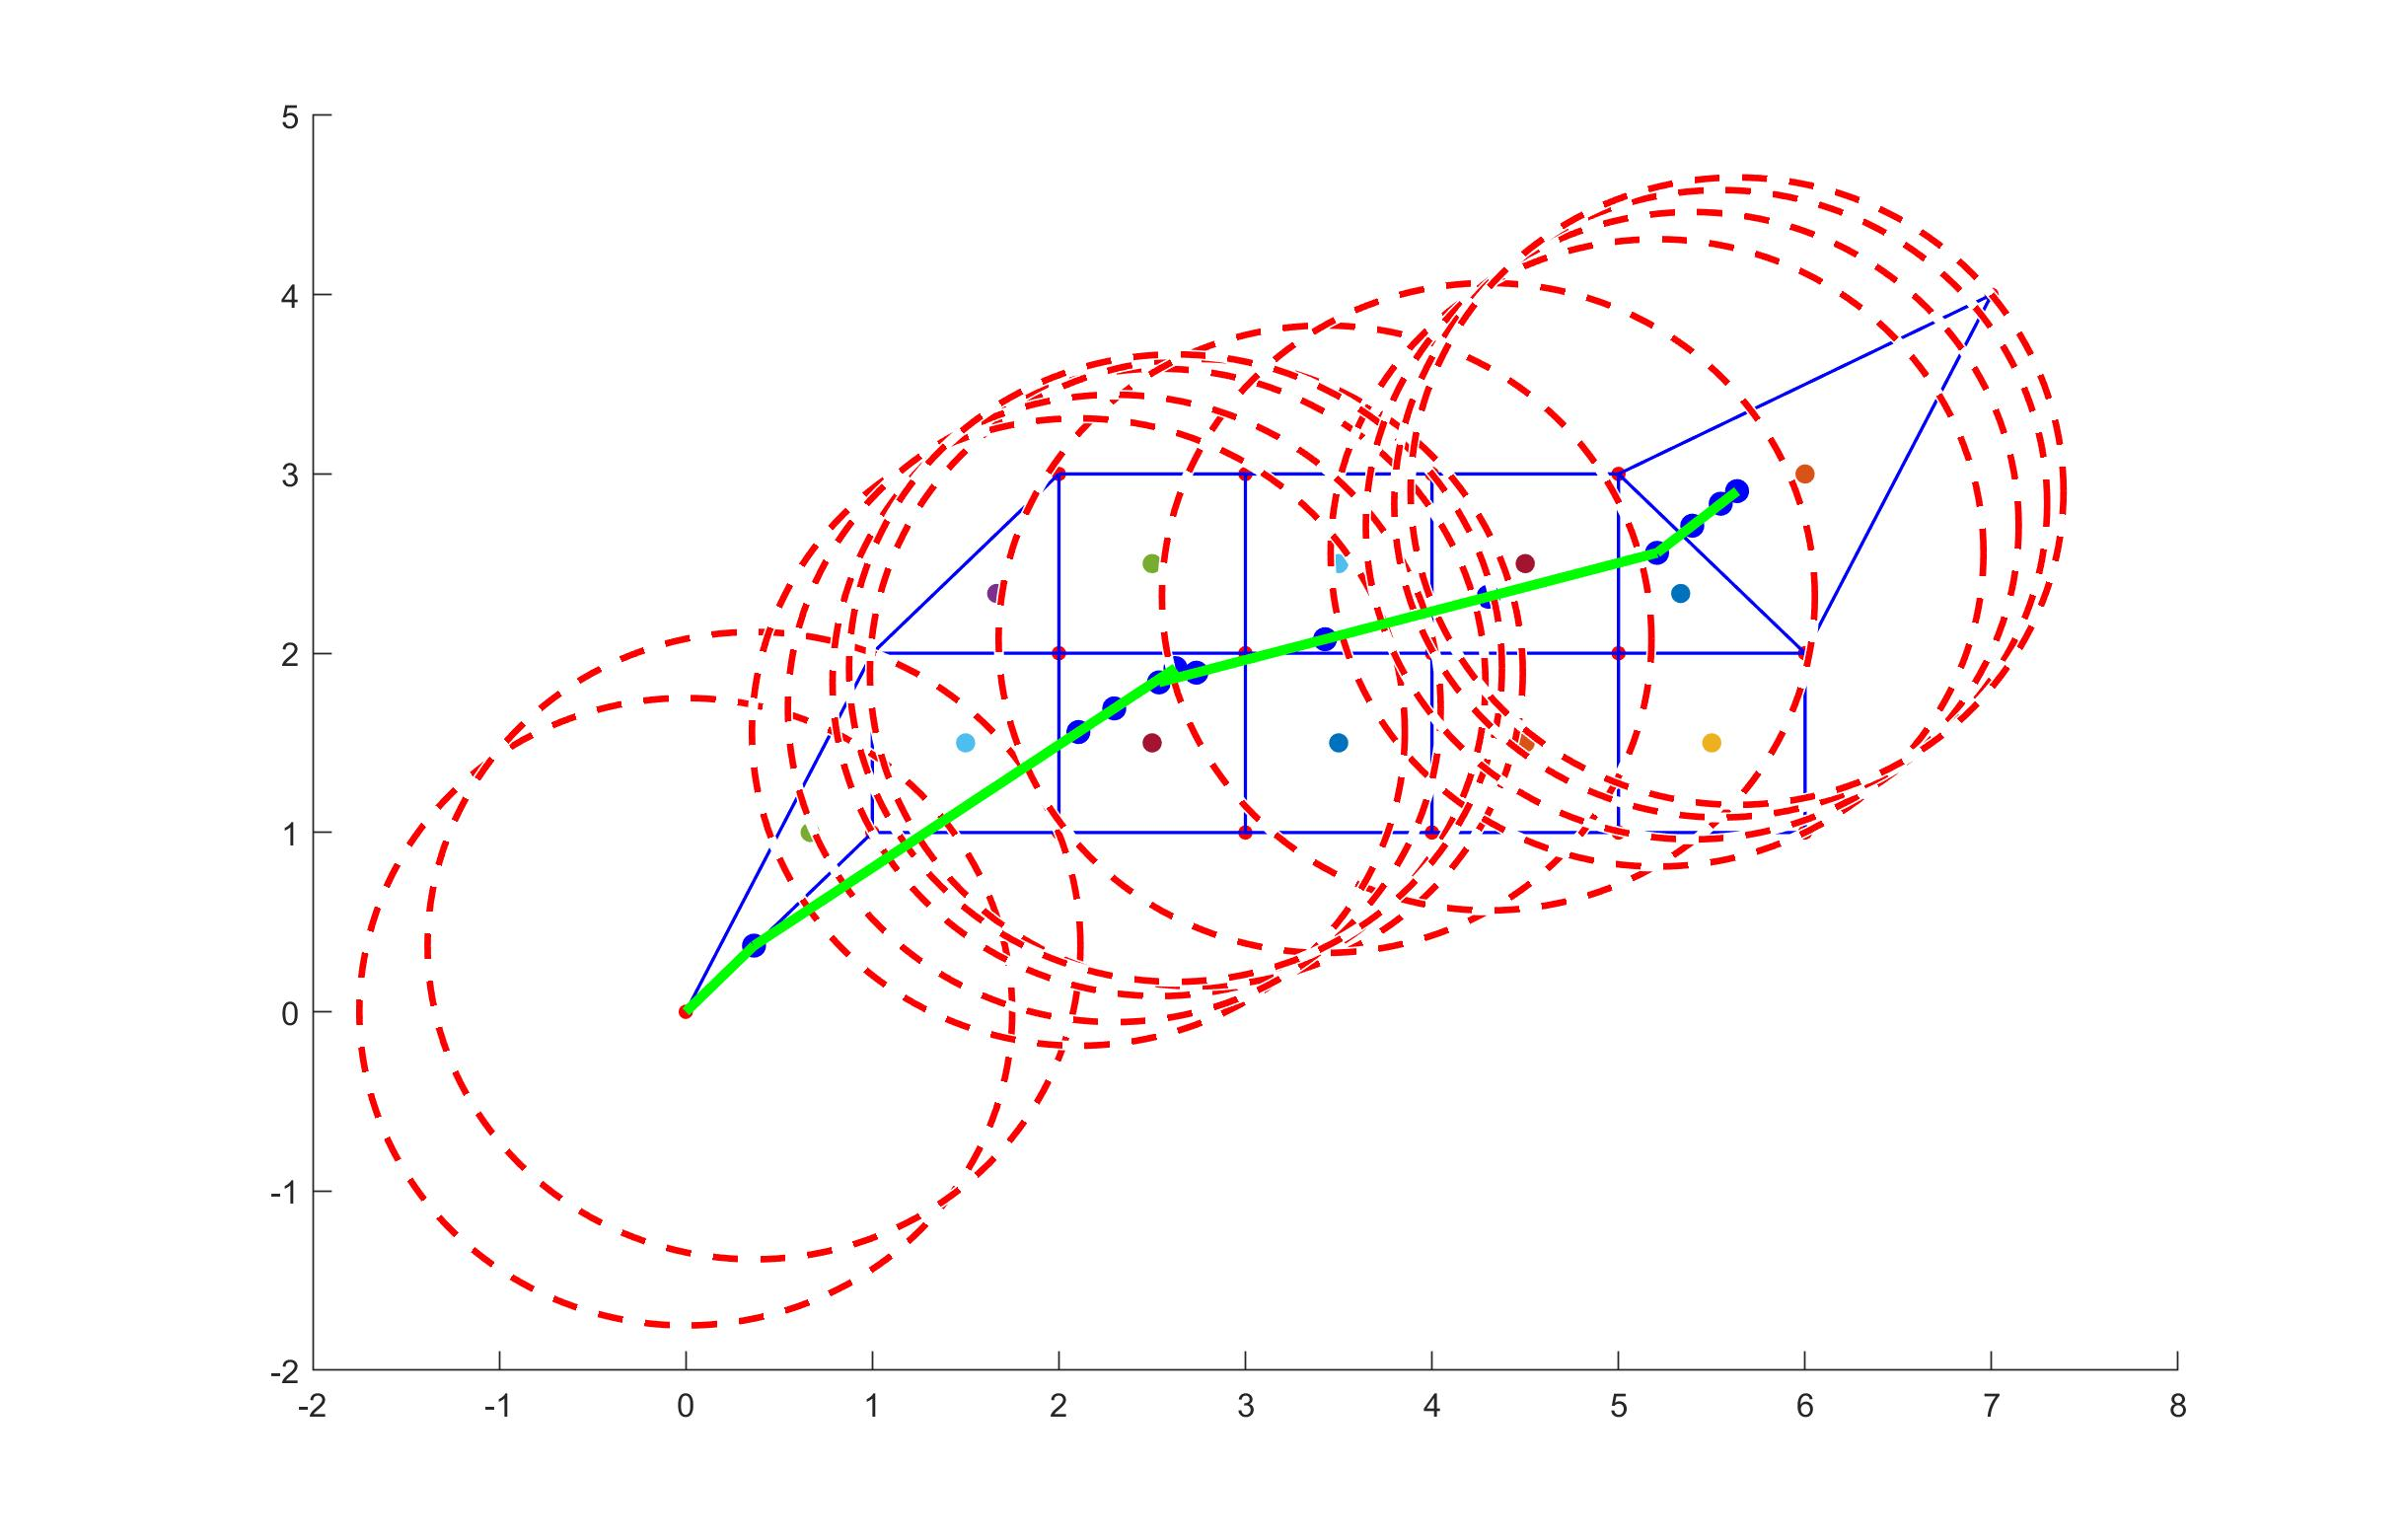
\includegraphics[height=1.6 true in]{Complete_Post.jpg}}
    \vskip -0.1 true in
    \caption{Twelve square and triangular cell boundaries are shown with blue lines.  The dash red
      circles represent the radius of coverage at each sensing node.  (a) Top: The green line
      represents the sensory coverage path found by applying Alg. \ref{alg:hoogeveen} to the nodes at the geometric
      center of each cell. (b) Bottom: The result of appyling
      Alg. \ref{alg:sensory_coverage} to optimize the sensing node locations.}
  \label{fig:complete_example}
  \vskip -0.2 true in
\end{figure}
\vspace{1mm}
%% ------------------------------ %%
%
{\bf Example:}  Fig. \ref{fig:complete_example} shows the action of Alg. \ref{alg:sensory_coverage} on a workspace divided into nonuniform convex cells.  Fig. \ref{fig:complete_example} depicts the initial un-optimized path through the cell centers, the optimized sensing locations, and the unpruned sensing nodes.  The solution  was computed in 0.8 second. \vspace{-1mm}

\subsection{Approximation Bound and Performance Analysis}

\noindent The concept of a {\em Cell Sensing Core} (Fig. \ref{fig:completecoverage}(a)) leads to an approximation bound for Alg. \ref{alg:sensory_coverage} directly from Prop. \ref{prop:bound1}.  To cover $\Cs_i$, the robot must pass through the $i^{th}$ cell's sensing core, denoted $\Cs^{core}_i$, a convex set. A {\em core sensing circle}, $\Cs^{circ}_i$, is inscribed in $\Cs^{core}_i$. Its radius is the {\em sensing overfill}: the excess sensing range that is not needed to cover the cell.  Thus, our shortest path complete sensory coverage problem {\em reduces exactly to the covering path problem} of Sections \ref{sec:covering_path} and \ref{sec:polynomial}, with $\Cs^{core}$ replacing the sensory coverage circle.  

\begin{prop} \label{prop:final}
Let a polygonal workspace be decomposed into convex polygons.  For small sensing overfill, Alg. \ref{alg:sensory_coverage} produces in time $\Os(n^4)$ a complete sensory covering path whose approximation ratio satisfies Eqs (\ref{eq:bound_odd}) and (\ref{eq:bound_even}).  For large sensing overfills, the path length is bounded by $(5/3)$ times the length of the optimal TSP path through the cell centers.
\end{prop}
\noindent{\bf Proof sketch:} When the sensing overfill is less than the largest dimension of the smallest cell, the core sensing circles of different cells do not overlap. Then Prop. \ref{prop:bound1} applies.  With large sensing overfill, the cell sensing cores may overlap, and we must default to the performance limit of Prop. \ref{prop:bound_overlap}.

%%% ------------------------------------------------------------------------- %%
\section{Conclusions and Future Work} \label{sec:conclusions}

\noindent By studying the practical problem of multi-target sensory covering paths, we uncover the optimization structure underlying many sensory coverage problems, including complete sensory coverage.  This structure allowed us to produce efficient and flexible approximation algorithms with excellent performance. We are quite confident that our formulation will lead to analogous 3-dimensional sensory coverage results, and new algorithms that take account of sensor uncertainty and vehicle dynamics in the coverage planning process.

%%% ------------------------------------------------------------------------- %%
{\bf Acknowledgement}. This work was supported in part by DARPA through the Subterranean Challenge program and by a grant from Beyond Limits and BP Inc. to the Calteh Center for Autonomous Systems and Technologies.

%%%%%%%%%%%%%%%%%%%%%%%%%%%%%%%%%%%%%%%%%%%%%%%%%%%%%%%%%%%%%%%%%%%%%%%%%%%%%%%%
\bibliography{Coverage,CoveringTour}
\bibliographystyle{unsrt}
%\bibliographystyle{ieeetr}
\end{document}
%%%%%%%%%%%%%%%%%%%%%%%%%%%%%%%%%%%%%%%%%%%%%%%%%%%%%%%%%%%%%%%%%%%%%%%%%%%%%%%%

